\documentclass{a0poster}
\usepackage{fancytikzposter} 
\usepackage[utf8]{inputenc}
\usepackage{amsmath}
\usepackage{amssymb}
\usepackage{listings}
\usepackage{zref-savepos}
\usepackage{minted}

%%%%% --------- Change here if you want ---------- %%%%%
%% margin for the geometry package, must be changed before using the geometry package
%% default value is 4cm
% \setmargin{4}

%% the space between the blocks
%% default value is 2cm
% \setblockspacing{2}

%% the height of the title stripe in block nodes, decrease it to save space
%% default value is 3cm
% \setblocktitleheight{3}

%% the number of columns in the poster, possible values 2,3
%% default value is 2
% \setcolumnnumber{3}

%% the space between two or more groups of authors from different institutions
%% used in \maketitle
% \setinstituteshift{10}

%% which template to use
%% N1 simple, standard look, with a colored background and gray boxes
%% N2 board with nodes
%% N3 another standard look
%% N4 envelope-like look
%% N5 with a wave-like head, original idea taken from
%%%% http://fc09.deviantart.net/fs71/f/2010/322/1/1/scientific_poster_by_nabuy-d333ria.jpg
%\usetemplate{6}

%% components of the templates
%% (the maximal possible numbers are mentioned as the parameters)
% \usecolortemplate{4}
% \usebackgroundtemplate{5}
% \usetitletemplate{2}
% \useblocknodetemplate{5}
% \useplainblocktemplate{4}
% \useinnerblocktemplate{2}


%% the height of the head drawing on top 
%% applicable to templates N3, 4 and 5
% \setheaddrawingheight{14}


%% change the basic colors
%\definecolor{myblue}{HTML}{008888} 
%\setfirstcolor{myblue}% default 116699
%\setsecondcolor{gray!80!}% default CCCCCC
%\setthirdcolor{red!80!black}% default 991111

%% change the more specific colors
% \setbackgrounddarkcolor{colorone!70!black}
% \setbackgroundlightcolor{colorone!70!}
% \settitletextcolor{textcolor}
% \settitlefillcolor{white}
% \settitledrawcolor{colortwo}
% \setblocktextcolor{textcolor}
% \setblockfillcolor{white}
% \setblocktitletextcolor{colorone}
% \setblocktitlefillcolor{colortwo} %the color of the border
% \setplainblocktextcolor{textcolor}
% \setplainblockfillcolor{colorthree!40!}
% \setplainblocktitletextcolor{textcolor}
% \setplainblocktitlefillcolor{colorthree!60!}
% \setinnerblocktextcolor{textcolor}
% \setinnerblockfillcolor{white}
% \setinnerblocktitletextcolor{white}
% \setinnerblocktitlefillcolor{colorthree}




%%% size of the document and the margins
%% A0
% \usepackage[margin=\margin cm, paperwidth=118.9cm, paperheight=84.1cm]{geometry} 
\usepackage[margin=\margin cm, paperwidth=84.1cm, paperheight=118.9cm]{geometry}
%% B1
% \usepackage[margin=\margin cm, paperwidth=70cm, paperheight=100cm]{geometry}



%% changing the fonts
\usepackage{cmbright}
%\usepackage[default]{cantarell}
%\usepackage{avant}
%\usepackage[math]{iwona}
\usepackage[math]{kurier}
\usepackage[T1]{fontenc}


%% add your packages here
\usepackage{hyperref}





\title{Sharygin Triangles \& Cubic Curves}
\author{Gregor Maclaine, Mikolaj Syska, Evan Sverdlov, Craig Boswell \\
  University of Edinburgh
}


\begin{document}

%%%%% ---------- the background picture ---------- %%%%%
%% to change it modify the macro \BackgroundPicture
\ClearShipoutPicture
\AddToShipoutPicture{\BackgroundPicture}

\noindent % to have the picture right in the center
\begin{tikzpicture}
  \initializesizeandshifts
  % \setxshift{15}
  % \setyshift{2}


  %% the title block, #1 - shift, the default value is (0,0), #2 - width, #3 - scale
  %% the alias of the title block is `title', so we can refer to its boundaries later
  \ifthenelse{\equal{\template}{1}}{ 
    \titleblock{47}{1}
  }{
    \titleblock{47}{1.5}
  }

  %% a logo can be added to the title block
  %% #1 - anchor relative to the title block, #2 - shift, #3 - width, #3 - file name
  % \ifthenelse{\equal{\template}{2}}{ 
  %   \addlogo[south west]{(2,0)}{6cm}{unibz_b.png}
  % }{
  %   \addlogo[south west]{(2,0)}{6cm}{unibz_w.png}
  % }


  %% a block node, with the specified position (optional), title and the content
  %% #1 - where (optional), #2 - title, #3 - text
  %%%%%%%%%% ------------------------------------------ %%%%%%%%%%
  \blocknode%
  {What Are Sharygin Triangles}%
  {
    To understand what a Sharygin triangle is, we let $\Delta ABC$ be a triangle in $\mathbb{R}^2$ (Shown in Fig. \ref{fig:triangle}) and let $AD$, $BE$ and $CF$ be its angle bisectors. This will yield another triangle $\Delta DEF$. We then define $\Delta ABC$ to be a Sharygin triangle if $\Delta DEF$ is isosceles and $\Delta ABC$ is non-isosceles. Then let $AC = x$, $BC = y$ and $z = AB$, and through application of the angle bisector theorem: 
$$DF-EF = \left(x-y\right)\frac{xyz}{\left(x+y\right)\left(x+z\right)^2\left(y+z\right)^2}f_3\left(x,y,z\right).$$
Where 
$$f_3(x,y,z) = x^3 + x^2y + xy^2 + y^3 + z\left(y^2 + xy+x^2\right) - z^2\left(x + y\right) - z^3.$$
This equation ensures that $\Delta ABC$ is isosceles while also showing that $\Delta ABC$ is a Sharygin triangle strictly if $f_3(x,y,z)=0$ and $x\neq y$. 

    

    \begin{tikzfigure}[Labelled Triangle]
        \label{fig:triangle}
        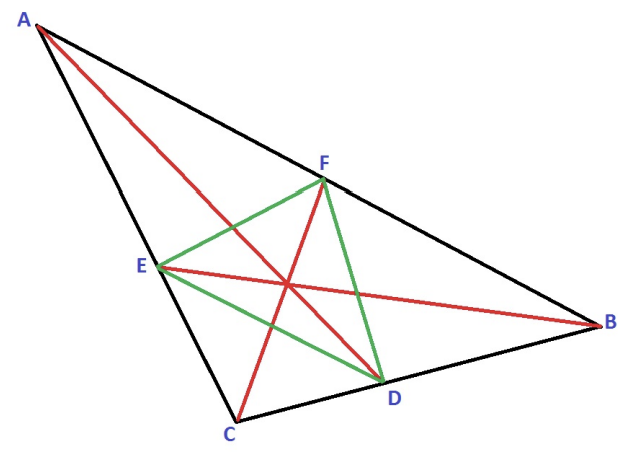
\includegraphics[width=0.4\linewidth]{Triangle.png}
    \end{tikzfigure}

}


  %%%%%%%%%% ------------------------------------------ %%%%%w[($(currenty)-(3.5,0)$)]{30}%%%%%
  \blocknode{The History} %
  { Sharygin triangles evolved from the Steiner-Lehmus Theorem and its geometric implications. It is a great example of the complex, interwoven nature of modern mathematics. 
 \hfill \break

Sharygin triangles owe their name to Igor Sharygin, a prolific Russian mathematician and mathematical educator, who investigated them in ``Problems in Plane Geometry''\cite{number9}. Unfortunately, despite his contributions to mathematics, he was forced to resign from Moscow State University due to his anti-Soviet political beliefs. 
The results of algebraic geometric explored in this poster are largerly a product of the search for Sharygin triangles with have integer-length sides. As will be shown in this poster, such triangles exist (and there are infinitely many of them). Sergei Markelov aimed to create a computer algorithm that would find integer-length Sharygin triangles with side length not exceeding a million but after two months of computations, the algorithm failed to find any. The search for Sharygin triangles led to many novel results in projective geometry.
}



  %% by default, the position of the new block node is right below the previous
  %% block node, stored in (currenty)
  %% box is the alias of the previous block, so we can refer to its boundaries

  %%%%%%%%%% ------------------------------------------ %%%%%%%%%%
  \blocknode{How Many Sharygin Triangles Are There?}%
{  As indicated in ``Plotting the Cubic Curve'' each point in the subset of the cubic curve $C$ defined by the triangle inequalities corresponds to a unique Sharygin triangle. Therefore, determining the number of pairwise non-similar Sharygin triangles with integer sides would be equivalent to determining the number of rational points in the considered subset of the cubic curve (because they can be scaled up as to have integer sides). It turns out that there are infinitely many of them. The proof of this statement can be found in \cite{number5} and it requires some advanced mathematical results that we could not illustrate here. 
\hfill \break

However, for a better intuitive understanding of the topic we describe an intermediate result, namely that there are infinitely many rational points on the elliptic curve in question (although that does not directly imply that there are infinitely many rational points in any specific subset of the curve).
\hfill \break

The first step is noting that point $A = (1 : 0 : −1)$ has infinite order. By computing $A, 2A,\ldots, 12A$ we can verify that neither of those points is equal to the chosen identity point $O = (1 : -1 : 0)$, therefore, by Mazur’s Theorem, point $A$ has to have infinite order. This result and the fact that the point $A$ is rational, allows us to construct infinitely many rational points lying in the cubic curve $C$. This is owing to the fact that adding two rational points on an elliptic curve will always result in another rational point, and it is not difficult to see why. 
\hfill \break

Consider the equation of the elliptic curve $E$ in $U_z$  formed from the cubic equation $C$ by a projective transformation. Firstly, every line passing through 2 rational points in $\mathbb{R}^2$ must have rational coefficients. Also, a line that is tangent to the curve $E$ at a rational point must have a rational gradient, and hence rational coefficients. Finding intersection points of a line with rational coefficients and $E$ would correspond to solving a cubic equation with rational coefficients. Since, we know that 2 of its roots (counting multiplicities) are rational, from Vieta’s formulas it follows that the 3rd root must also be rational (if a sum of 2 numbers of which one is rational is rational, the second one must also be rational). Keeping in mind how addition on cubic curves is defined, the above implies that adding two rational points on an elliptic curve will always result in another rational point. Since point A has infinite order and is rational, for all $n \in \mathbb{N}$, $nA$ is a unique rational point. Therefore, there are infinitely many rational points on $C$. As shown in \cite{number5} these points are dense on $C$, thus, there are infinitely many of them in any subset of $C$.
}


  %%%%%%%%%%%%% NEW COLUMN %%%%%%%%%%%%%%% 
  \startsecondcolumn 

  
  %%%%%%%%%% ------------------------------------------ %%%%%%%%%%
  \blocknode{Plotting the Cubic Curve}%
  { We can identify $U_z$ with $\mathbb{C}^2$ with coordinates $\bar{x} = \frac{x}{z}$ and $\bar{y} =\frac{y}{z}$.
Then $\mathbb{C} \cap U_z$ is a cubic curve in $\mathbb{C}^2$
that is given by

$$\bar{x}^3+\bar{x}^2\bar{y} + \bar{x}\bar{y}^2+\bar{y}^3+\bar{y}^2+\bar{x}\bar{y}+\bar{x}^2-\bar{x}-\bar{y}-1=0.$$

Using Python, we can plot its real part:

    \begin{tikzfigure}[The Cubic Curve at z=1 overlapping with the Triangle Inequality.]
        \label{fig:cubiccurve}
        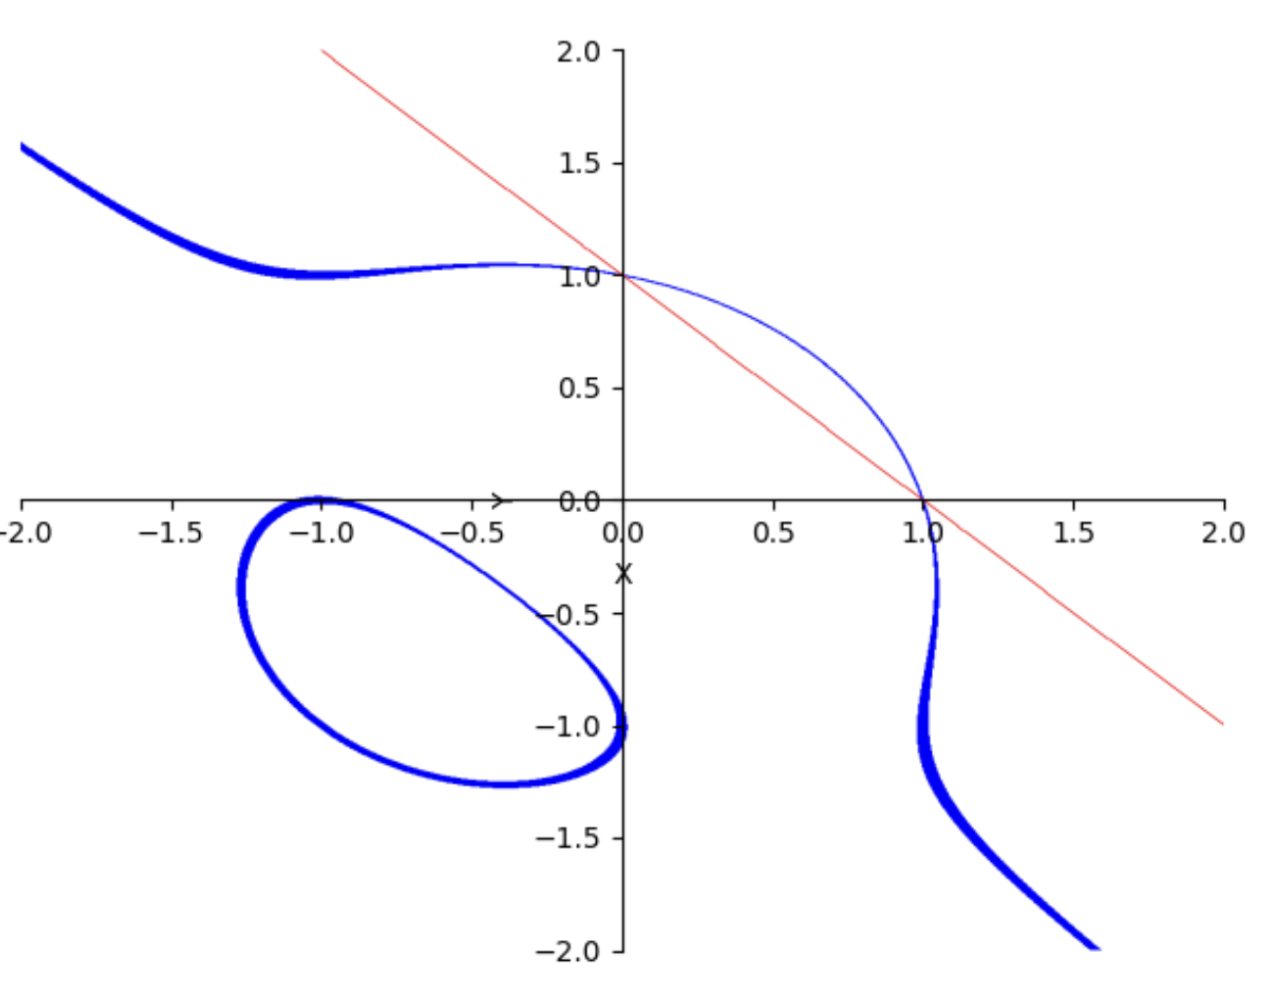
\includegraphics[width=0.4\linewidth]{Diagram.png}
    \end{tikzfigure}

  In this figure, the triangle inequality is shown as all points above the red line. Because every triangle has to satisfy the triangle inequalities, Sharygin triangles (up to similarity) are points in the subset of the cubic curve defined by the triangle inequalities, which is the part curve lying above the red line in figure above.

  }
   %%%%%%%%%%%%% NEW COLUMN %%%%%%%%%%%%%%% 
  %% (if column number is 3)
  \startthirdcolumn

  %%%%%%%%%% ------------------------------------------ %%%%%%%%%%
  \blocknode {How To Generate A Triangle With Integer Sides}%
  {
  % \lstinputlisting[language=Python,basicstyle=\normalsize,xleftmargin=1cm]{code.py}

\inputminted{Python}{code.py}



  Using the algorithm defined in \cite{thebook}, this code yields the triangle generated by $8\left[1:0:1\right]$:  $$\left[
  301361533449900458837600 : \\
      49105016933436320224063 : \\
         316629033253501281102807
 \right]$$
  }



  \blocknode {References}%
  {
  
\fontsize{26}{26}\selectfont  % Change the font size for the references
\begin{thebibliography}{9}
% A journal article
\bibitem{number5}
I. Netay, A. Savvateev, \emph{Sharygin triangles and elliptic curves.}
Magadan Volume, Bulletin of the Korean Mathematical Society 54 (2017) 1597–1617

% A textbook
\bibitem{thebook}
I. Cheltsov, \emph{Algebraic Geometry for sophomores.}
Learn, University of Edinburgh, 2019

\bibitem{number9}
I. Sharygin, \emph{Problems in Plane Geometry.}
Mir Publishers, 1988

\end{thebibliography}
  }



\end{tikzpicture}


\end{document}
